\section{Metodologia e Abordagens}

% Elaborar nesta seção a descrição das abordagens de solução, incluindo:
% 1. Método exato (MIP) para o problema bi-objetivo/eps-restrito
% 2. Heurísticas (construtivas e de melhoria) para o problema bi-objetivo/eps-restrito
% 3. Metaheurística NSGA-II para o problema bi-objetivo/eps-restrito, incluindo:
%    - Operadores mais impactantes
%    - Estratégia "Compacto" vs. "Expandido" para o encoding
% Fonte: docs/refs/dissertacao_tex/2-textual/heuristicas.tex
% Arco: eps-restrito -> MIP-heurísticas -> NSGA-II -> operadores -> encoding -> síntese.

%%% Frame 3.1 — Bi-objetivo + eps-restrito (TikZ Pareto)
\begin{frame}{Abordagem bi-objetiva: método \(\varepsilon\)-restrito}
    \begin{columns}[c]
        \begin{column}{0.54\textwidth}
            Objetivos conflitantes \(\rightarrow\) \textbf{fronteira de Pareto} \cite{Haimes_Wismer_1971}.
            \begin{itemize}
                \item \(Z_1\) como objetivo; \(Z_2 \leq \varepsilon\) como restrição.
                \item Limites por otimização lexicográfica.
                \item Grade de \textbf{7 pontos} \(\varepsilon\) por instância \cite{Saez-Aguado_Trandafir_2018}.
            \end{itemize}
        \end{column}
        \begin{column}{0.46\textwidth}
            \centering
            \begin{tikzpicture}[scale=0.82]
                \draw[->] (0,0) -- (4.3,0) node[right]{\footnotesize \(Z_1\)};
                \draw[->] (0,0) -- (0,3.5) node[above]{\footnotesize \(Z_2\)};
                \draw[very thick,UFTblue] (0.45,3.1) .. controls (1.1,0.95) and (2.1,0.65) .. (3.9,0.38);
                \foreach \y in {0.6,1.1,1.6,2.1,2.6} {\draw[dashed,UFTgray] (0,\y) -- (4.0,\y);}
                \foreach \p in {(0.6,2.6),(0.78,2.1),(1.12,1.6),(1.75,1.1),(3.05,0.6)}
                    {\fill[PROFMATgreen] \p circle (2.2pt);}
                \node[UFTgray] at (3.3,2.35){\tiny \(Z_2 \leq \varepsilon\)};
            \end{tikzpicture}
        \end{column}
    \end{columns}
    % TODO: grade compartilhada por todos os métodos MIP (comparabilidade ponto a ponto).
\end{frame}

%%% Frame 3.2 — MIP-heurísticas (TikZ janela deslizante)
\begin{frame}{MIP-heurísticas: decomposição temporal}
    \begin{center}
        \begin{tikzpicture}[scale=0.9]
            \foreach \i in {0,...,6} {
                \draw[fill=UFTgray!15] (\i,0) rectangle (\i+0.85,0.6);
            }
            \fill[UFTgreen!45] (2,0) rectangle (2.85,0.6);
            \fill[UFTgreen!45] (3,0) rectangle (3.85,0.6);
            \node[below] at (1.0,-0.05){\footnotesize fixado};
            \node[below] at (3.35,-0.05){\footnotesize janela \((d,t)\)};
            \node[below] at (5.7,-0.05){\footnotesize relaxado};
        \end{tikzpicture}
    \end{center}
    \vspace{0.4em}
    \begin{itemize}
        \item \textbf{Relax-and-Fix} (construtiva): resolve a janela, fixa \(w_{iud}\), avança.
        \item \textbf{Fix-and-Optimize} (melhoria): fixa fora da vizinhança, reotimiza.
        \item \textbf{Híbrido} RF~\(\rightarrow\)~FO: constrói e depois refina \cite{Turhan_Bilgen_2020}.
    \end{itemize}
\end{frame}

%%% Frame 3.3 — NSGA-II base (figura fluxo principal)
\begin{frame}{Meta-heurística: NSGA-II}
    \footnotesize
    Base evolutiva \cite{Deb_Pratap_Agarwal_Meyarivan_2002}:
    \begin{itemize} % TODO : itens lado a lado
        \item Ordenação não-dominada. \quad \item Distância de \textit{crowding}. \quad \item Elitismo (pais \(\cup\) filhos).
    \end{itemize}
    
    \begin{figure}
        \centering
        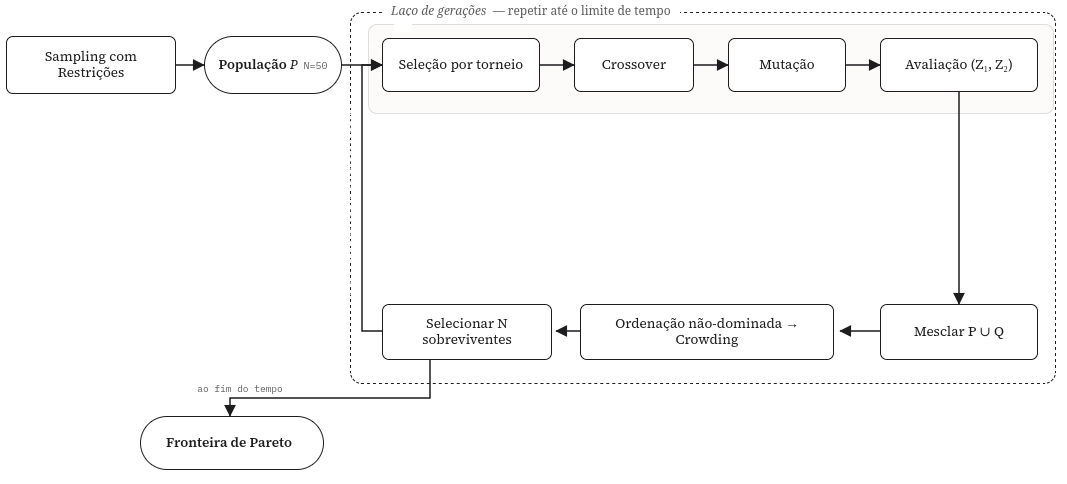
\includegraphics[width=\linewidth]{img/04_nsga-01_laco-principal.png}
        \caption{Fluxo principal do NSGA-II.}
        \label{fig:nsga-loop}
    \end{figure}
\end{frame}

%%% Frame 3.4 — Operadores customizados (2 figuras complementares)
\begin{frame}{Operadores customizados}
    Amostragem inicial \textbf{com consciência de restrições} \(+\) dois operadores que preservam a coerência temporal da agenda:
    \begin{columns}[T]
        \begin{column}{0.5\textwidth}
            \begin{figure}
                \centering
                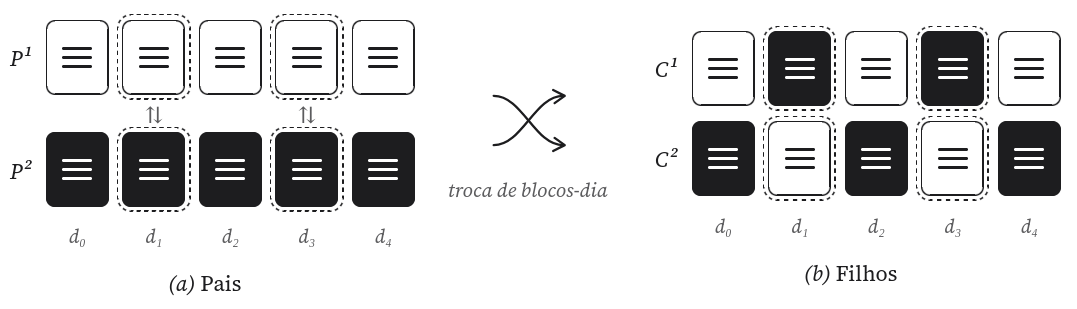
\includegraphics[width=\linewidth]{img/02_crossover.png}
                \caption{\footnotesize Cruzamento por blocos diários.}
            \end{figure}
        \end{column}
        \begin{column}{0.5\textwidth}
            \begin{figure}
                \centering
                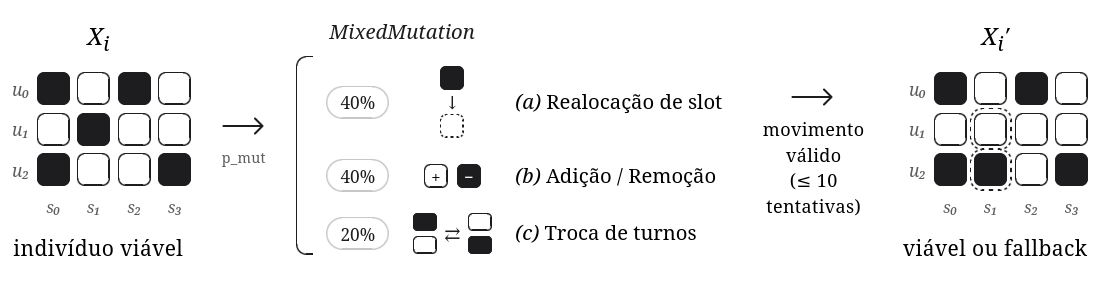
\includegraphics[width=\linewidth]{img/03_mutacao.png}
                \caption{\footnotesize Mutação por realocação de \textit{slot}.}
            \end{figure}
        \end{column}
    \end{columns}
\end{frame}

%%% Frame 3.5 — Encoding Compacto vs Estendido
\begin{frame}{Codificação: Estendido \emph{vs.} Compacto}
    \begin{figure}
        \centering
        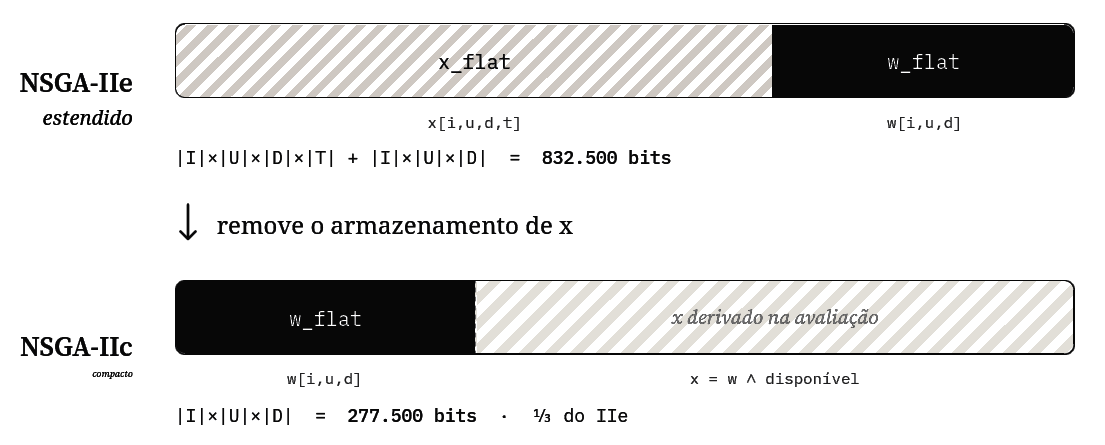
\includegraphics[width=0.82\linewidth]{img/05_encoding.png}
        \caption{Comparação dos \textit{encoders}.}
        \label{fig:encoding}
    \end{figure}
    \begin{itemize}
        \item \textbf{Estendido:} \(x_{iudt}\) e \(w_{iud}\) binários \(\rightarrow\) alta dimensionalidade.
        \item \textbf{Compacto:} gene por médico--dia (\(\approx w\)) \(\rightarrow\) \(\sim\)70\(\times\) menor, mais gerações.
    \end{itemize}
\end{frame}

%%% Frame 3.6 — Síntese das três famílias (transição p/ resultados)
\begin{frame}{Síntese: três famílias de solução}
    \begin{center}
        \begin{tabular}{lccc}
            \toprule
            & \textbf{Exato} & \textbf{MIP-heur.} & \textbf{NSGA-II} \\
            \midrule
            Garante factibilidade & sim & sim & parcial \\
            Escalabilidade (90 d) & baixa & média & alta \\
            Soluções por execução  & 7 (grade) & 7 (grade) & \(\sim\)100 \\
            \bottomrule
        \end{tabular}
    \end{center}
    \vspace{0.6em}
    \centering{\footnotesize Trade-offs distintos \(\rightarrow\) avaliados nos experimentos a seguir.}
\end{frame}
